\chapter{基于几何约束的策略学习方法}
第三章围绕智能体强化学习在复杂环境中的安全性问题，构建了基于约束流行的安全过滤机制，在一定程度上缓解了机器人在运动过程中的风险行为。然而，在多机器人协同任务中，系统不仅需要满足个体层面的安全可行性，还需在群体层面同时维持编队拓扑、相对位姿关系与任务协同效率，这使得控制目标由单一安全约束扩展为多任务耦合下的结构化优化问题。

基于此，第四章在第三章安全约束思想的基础上进一步强化与拓展，将安全约束从个体避碰推广至多机器人几何关系保持，使强化学习策略能够在满足安全边界的前提下，更有效地利用编队结构先验实现协同决策。由此，本章旨在继承第三章安全保证能力的同时，提升多机器人系统在复杂任务中的组织性、稳定性与控制性能。
\section{方法框架}
本文提出一种基于几何约束的策略学习方法（Geo-Constrained Policy Learning, GCPL），
通过融合强化学习与几何结构约束，实现多机器人系统在复杂环境中的安全协同与编队控制，系统整体控制流程可划分为候选动作生成、安全修正、解析合成、环境交互以及策略更新五个阶段。
\begin{figure}
    \centering
    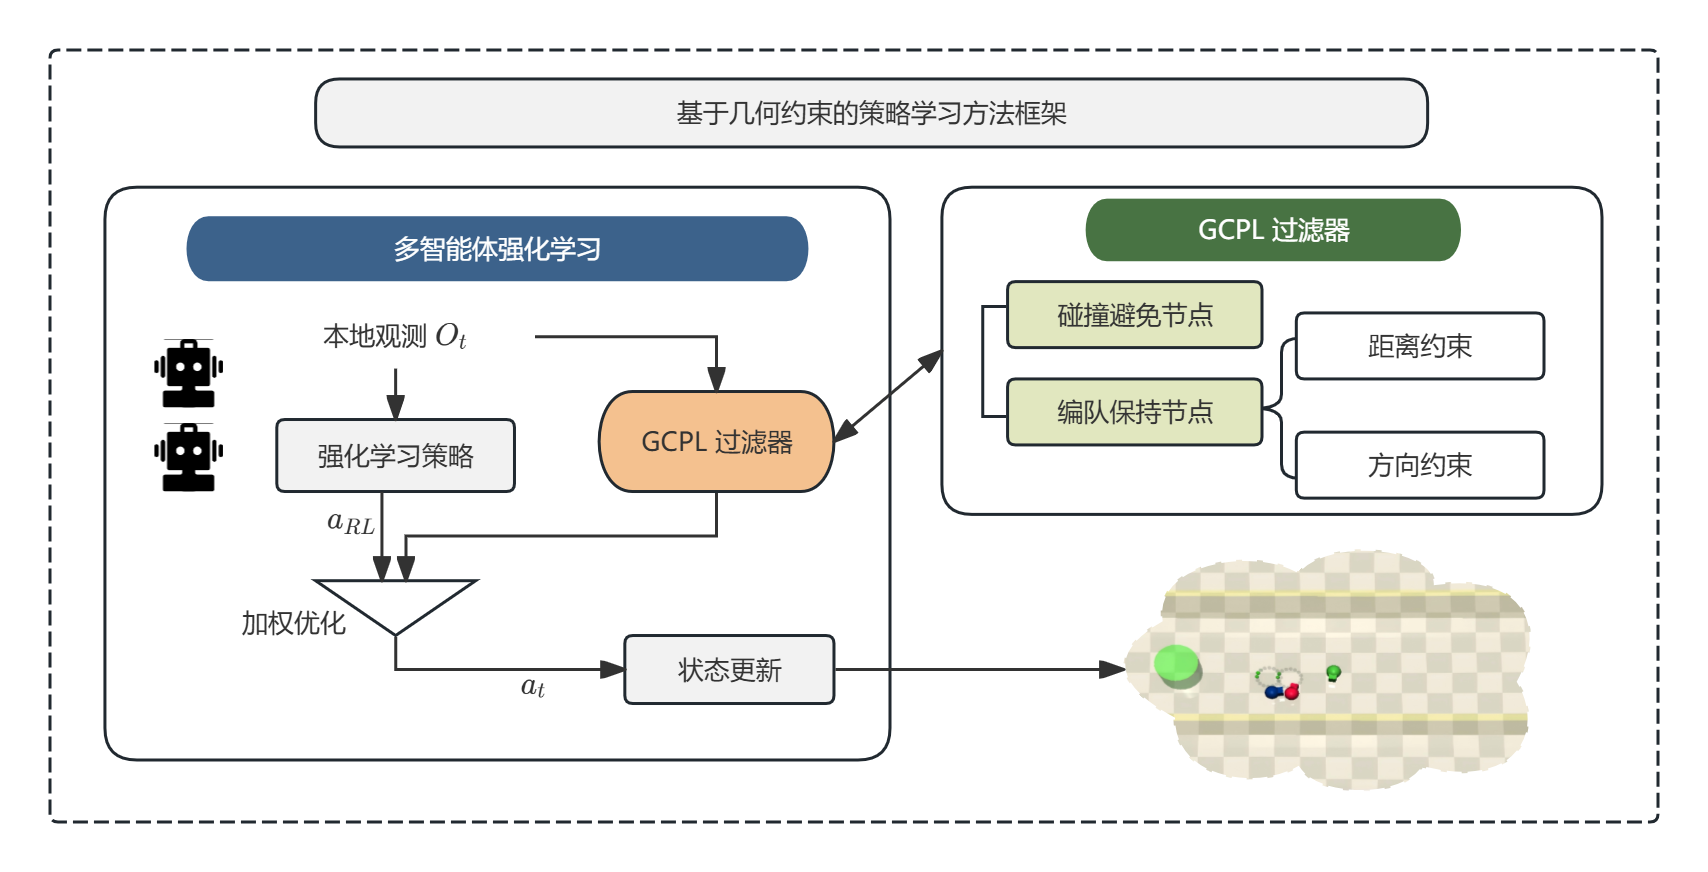
\includegraphics[width=1\linewidth]{images/RMPflow framework.png}
    \caption{GCPL 算法框架}
    \label{fig:RMPflow framework}
\end{figure}
在强化学习层，本文采用基于策略梯度的近端策略优化方法构建多智能体策略网络（Multi-Agent Proximal Policy Optimization，MAPPO）。策略网络以系统在时刻 $x_t$ 的观测状态作为输入，输出一个候选控制动作 $a^{RL}$。该候选动作主要反映任务层面的优化需求，包括尽可能缩短到达目标的时间、提升通过复杂区域时的效率以及维持更合理的编队形态等，但在这一阶段并未对机器人之间的安全距离或障碍物约束进行严格保证，因此其结果更多体现为策略在当前状态下给出的原始控制意图。

在几何过滤层，引入基于黎曼流形运动策略表示的控制框架，对强化学习产生的候选动作进行约束与融合。在该框架中，系统被组织为一棵任务树，树中每一个叶节点都对应一个具有明确几何含义的子任务，例如目标跟踪、障碍物规避、速度范围限制以及机器人之间的安全间距维持等。每个任务都以自然形式 $(f_i, M_i)$ 表示，其中 $f_i$ 描述任务空间中的期望控制动作，$M_i$ 则作为度量矩阵，用来刻画该任务在局部几何结构中的重要程度以及不同方向上的权重分布。强化学习输出的候选动作 $a^{RL}$ 在这一结构中被建模为一个额外的叶节点任务，并与其他安全相关任务共同参与后续的合成过程，使其影响受到整体几何约束的调节，而不是直接作用于系统。

在GCPL的计算过程中，各叶节点首先通过推前映射在各自的任务空间中完成评估，随后在拉回阶段通过雅可比映射被统一投影回根节点所在的空间。所有叶节点的自然形式在同一坐标框架下进行叠加，得到整体的广义力与度量矩阵：
\begin{equation}
(f_{total}, M_{total}) = \sum_i Pullback(f_i, M_i).
\end{equation}
这一过程本质上是在统一的几何度量下对多个任务进行一致性整合，使得不同任务在系统状态变化时能够通过各自的度量矩阵自动调整权重。当某一约束在当前情形下更为关键时，其对应的度量值会明显增大，从而在合成结果中产生更强的影响，而其他任务的作用则相对减弱，这样可以在不引入硬切换的情况下缓解任务之间的冲突。

当所有任务信息汇总至根节点之后，系统通过解析步骤计算最终的控制输出：
\begin{equation}
a = M_{\text{total}}^{\dagger} f_{total},
\end{equation}
其中 $M_{\text{total}}^{\dagger}$ 表示度量矩阵的广义逆。该求解过程可以理解为在整体度量约束下，对各个任务期望进行加权后的最小二乘意义最优解。由此得到的加速度指令既包含了强化学习层所提供的任务驱动趋势，又在数值上受到安全相关任务的修正与限制，使其在满足几何一致性的同时保持物理上可实现。

机器人按照该安全修正后的控制量与环境进行交互，并转移到下一时刻的状态。环境根据编队保持情况、到达目标的效率以及是否违反安全约束等因素生成奖励信号 $r_t$，这一信号被反馈给 MAPPO 策略网络，用于更新策略参数。随着训练的不断推进，策略逐渐学会在其可行动作范围内输出更符合安全几何结构的控制意图，使得 GCPL 在在线修正时所需的调整幅度逐步减小，从而提升整体控制过程的平滑性与执行效率。
\begin{figure}
    \centering
    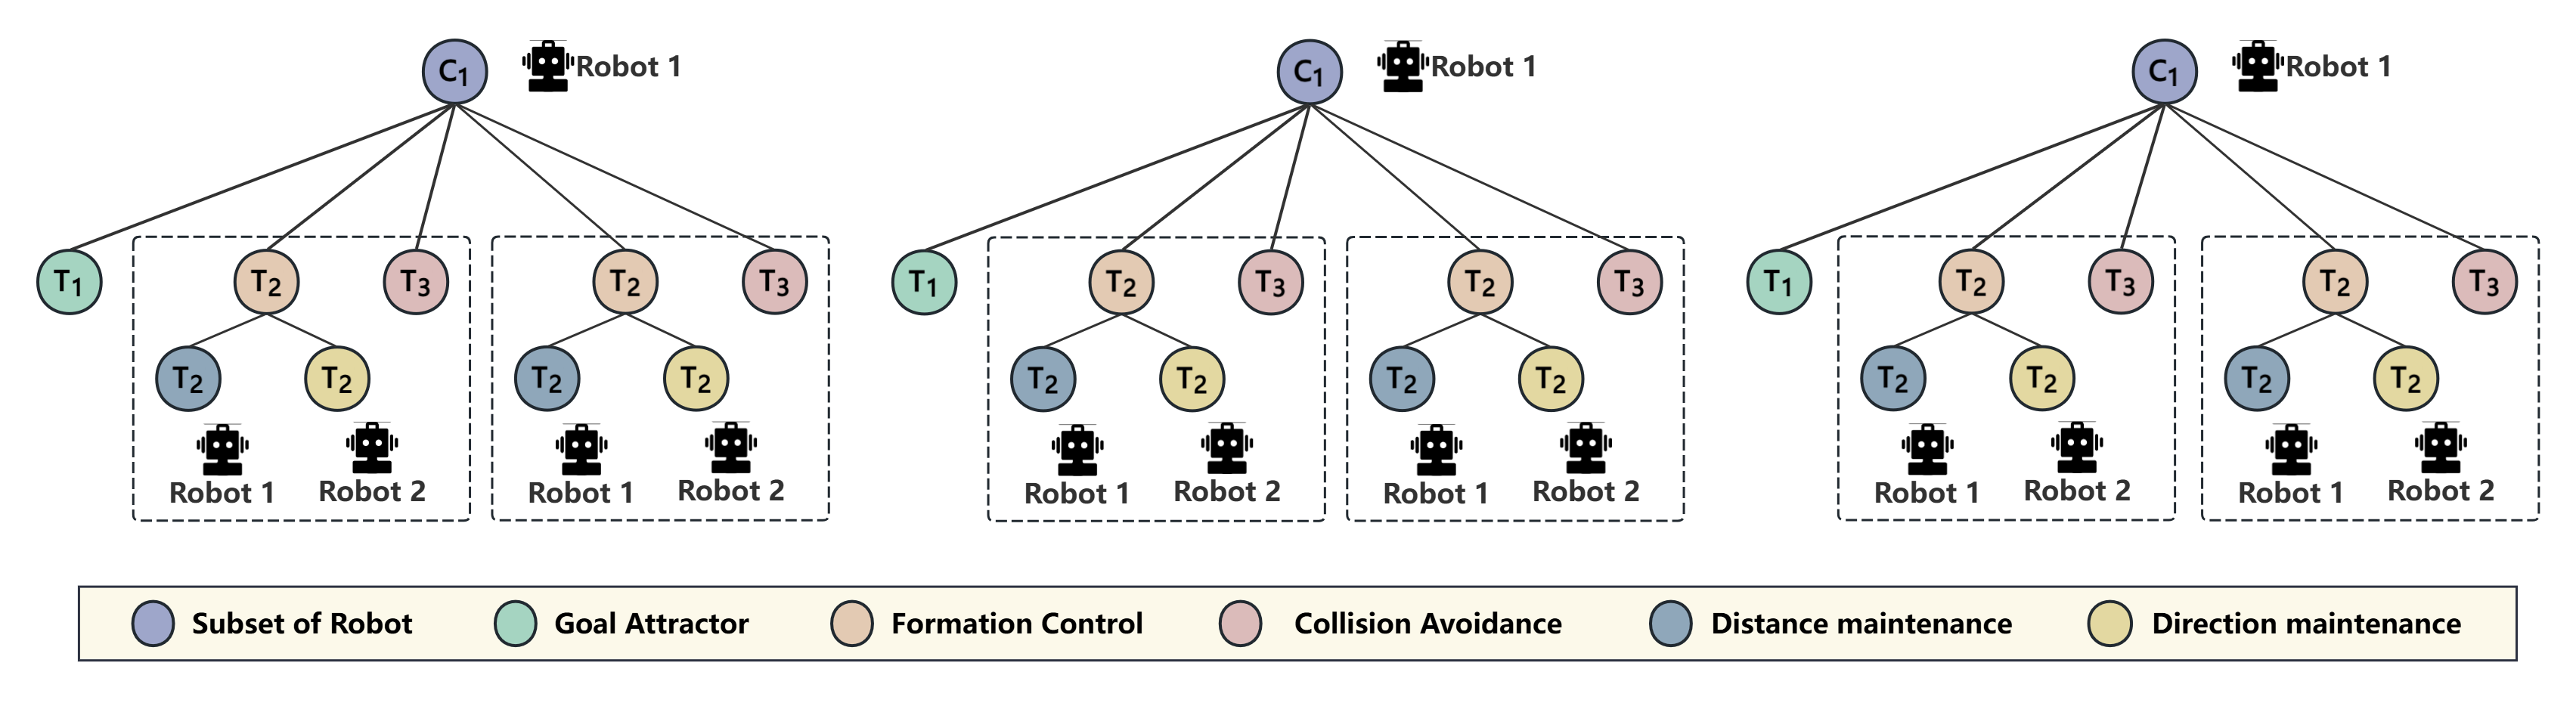
\includegraphics[width=1\linewidth]{images/rmpflow (1).png}
    \caption{GCPL任务树}
    \label{fig:RL-RMPflow树}
\end{figure}

\begin{algorithm}[t]
\caption{ GCPL 多机器人控制}
\label{alg:rl_rmpflow_simple}
\begin{algorithmic}[1]
\REQUIRE 多机器人初始状态 $x_0$，目标 $x_{\text{goal}}$，MAPPO 策略 $\pi_\theta$，几何任务集合 $\mathcal{T}$
\FOR{每个训练回合}
    \STATE 初始化环境与机器人状态 $x \leftarrow x_0$
    \FOR{每个时间步 $t$}
        \STATE \textbf{强化学习层：}每个机器人采样动作 $a^{RL}_{i,t} \sim \pi_\theta(o_{i,t})$
        \STATE \textbf{几何过滤层：}构建 RL 叶子节点和避障、编队任务节点
        \STATE 执行 pullback 及 合并：
        \[
        M_i = \sum_k M_{i,k}, \quad f_i = \sum_k f_{i,k}, \quad \ddot{x}_i = M_i^{-1} f_i
        \]
        \STATE 应用控制 $a_i$ 推进环境，计算奖励 $r_t$ 和代价 $c_t$
        \STATE 存储轨迹 $(o_t, a_t, r_t, c_t)$
    \ENDFOR
    \STATE 通过 MAPPO 更新策略参数 $\theta$
\ENDFOR
\end{algorithmic}
\end{algorithm}

\section{系统建模}
\subsection{状态与控制输入建模}
本文研究对象为工作在二维平面环境下的多差速移动机器人系统。为便于在 GCPL 框架下进行统一的几何力学建模与控制，首先对单个机器人进行状态与控制输入建模。
设机器人系统由若干个同构差速机器人组成，第 i 个机器人在平面内的配置空间状态可表示为机器人在世界坐标系下的平面位置坐标，以及当前航向角：
\begin{equation}
    q_i = (x_i,y_i,\theta_i)
\end{equation}

机器人的底层控制输入为前进线速度与转向角速度：
\begin{equation}
    u_i=(v_i,ω_i)
\end{equation}

GCPL 是在配置空间加速度层进行多任务融合的几何控制框架，本文将机器人控制问题建模为加速度级指令生成问题，即：
\begin{equation}
    \ddot{q_i} = a_i
\end{equation}
其中 $a_i =(a_x ,a_y)$为机器人质心在世界坐标系下的二维期望加速度。通过后续的运动学映射，可将该加速度指令转换为差速机器人可执行的线加速度与角加速度。
\subsection{编队的图建模}

为刻画多机器人系统的空间编队结构，本文采用无向图对编队拓扑进行建模。设系统包含 $N$ 个机器人，其在二维平面中的位置表示为
\begin{equation}
    p = (p_0, p_1, \ldots, p_{N-1}), \quad p_i \in \mathbb{R}^2.
\end{equation}

定义编队拓扑图为
\begin{equation}
    \mathcal{G} = (\mathcal{V}, \mathcal{E})
\end{equation}
其中节点集合 $\mathcal{V} = \{0,1,\ldots,N-1\}$ 表示机器人个体，边集合 $\mathcal{E} \subseteq \mathcal{V} \times \mathcal{V}$ 表示需要维持相对几何约束的机器人对。对于每一条边 $(i,j) \in \mathcal{E}$，指定期望的相对距离 $d_{ij}^* > 0$。

基于该图结构，定义编队的距离约束为
\begin{equation}
    \|p_i - p_j\| = d_{ij}^*, \quad \forall (i,j) \in \mathcal{E}.
\end{equation}

为刻画编队偏离程度，引入边的距离误差函数
\begin{equation}
    z_{ij} = \psi(p_i, p_j) = \|p_i - p_j\| - d_{ij}^*.
\end{equation}

进一步地，定义整体编队误差能量函数为
\begin{equation}
    E(p) = \frac{1}{2} \sum_{(i,j)\in\mathcal{E}} 
    \left( \|p_i - p_j\| - d_{ij}^* \right)^2,
\end{equation}
该能量函数用于度量当前编队与目标编队之间的整体偏差。

仅依赖距离约束时，编队结构在欧氏变换（平移与旋转）下是不变的，即该约束仅能保证编队的刚性形状，而无法唯一确定其方向与朝向。因此，为消除由旋转和镜像引起的不确定性，本文进一步在图结构上引入方向约束。

对于每一条边 $(i,j) \in \mathcal{E}$，定义单位方向向量为
\begin{equation}
    \hat{r}_{ij} = \frac{p_j - p_i}{\|p_j - p_i\|},
\end{equation}
并设定对应的期望方向 $\hat{r}_{ij}^*$。由此定义方向误差为
\begin{equation}
    z_{ij}^{\theta} = 1 - \hat{r}_{ij}^\top \hat{r}_{ij}^*.
\end{equation}

结合距离与方向约束，可得到联合编队能量函数
\begin{equation}
    E_{\text{form}}(p) = 
    \frac{1}{2} \sum_{(i,j)\in\mathcal{E}} 
    \left[
    \alpha_d \left( \|p_i - p_j\| - d_{ij}^* \right)^2
    +
    \alpha_\theta \left( 1 - \hat{r}_{ij}^\top \hat{r}_{ij}^* \right)^2
    \right],
\end{equation}
其中 $\alpha_d, \alpha_\theta > 0$ 分别为距离约束与方向约束的权重系数。

该图建模方法为后续编队保持节点的构建提供了统一的几何表示，同时也为强化学习奖励函数的设计提供了理论基础。

\subsubsection{不同编队形状的图结构构造}

在上述统一图建模框架下，不同编队形状可通过设计不同的边集合 $\mathcal{E}$ 及对应的期望距离 $d_{ij}^*$ 来实现。下面给出三种典型编队（直线、楔形和圆形）的图结构构造方法。

\paragraph{1) 直线编队（Line Formation）}

直线编队的目标是使机器人沿某一主轴方向排列，并仅维持相邻机器人之间的局部距离约束。设机器人按照索引顺序排列，则边集合定义为
\begin{equation}
    \mathcal{E}_{\text{line}} = \{ (i, i+1) \mid i = 0, 1, \ldots, N-2 \}.
\end{equation}

对应的期望距离通常设置为常数间距：
\begin{equation}
    d_{i,i+1}^* = d, \quad \forall (i,i+1) \in \mathcal{E}_{\text{line}}.
\end{equation}

该结构形成一条链式拓扑，仅约束局部相邻关系。由于该图不具备全局刚性，其整体朝向与宽度需要通过额外的方向约束或辅助奖励加以限制。

\paragraph{2) 楔形编队（Wedge Formation）}

楔形编队通常表现为以某一机器人为顶点的“V”字结构。设机器人 $0$ 为顶点，其余机器人分布在两侧，则边集合可构造为
\begin{equation}
    \mathcal{E}_{\text{wedge}} =
    \{ (0,i) \mid i = 1,\ldots,N-1 \}
    \cup
    \{ (i,j) \mid i,j \in \mathcal{N}_{\text{side}} \},
\end{equation}
其中 $\mathcal{N}_{\text{side}}$ 表示同侧机器人集合。

在实际实现中，可进一步为左右两侧分别定义不同的期望距离，以形成稳定的楔形夹角。例如，对于同一侧的相邻机器人：
\begin{equation}
    d_{ij}^* = d_{\text{side}}, 
\end{equation}
而对于顶点与侧边机器人：
\begin{equation}
    d_{0i}^* = d_{\text{apex}}.
\end{equation}

该结构通常构成刚性图，能够在二维平面中唯一确定编队形状（除整体刚体变换外）。

\paragraph{3) 圆形编队（Circle Formation）}

圆形编队的目标是使机器人均匀分布在一个圆周上。为此，可采用环形拓扑结构，即每个机器人仅与其相邻两个机器人建立连接：
\begin{equation}
    \mathcal{E}_{\text{circle}} =
    \{ (i, (i+1) \bmod N) \mid i = 0,1,\ldots,N-1 \}.
\end{equation}

对应的期望距离设置为相邻机器人在圆周上的弧长近似：
\begin{equation}
    d_{i,i+1}^* = 2R \sin\left(\frac{\pi}{N}\right),
\end{equation}
其中 $R$ 为期望圆半径。

\section{强化学习层}
强化学习层用于为多机器人系统提供目标导向的高层决策与性能优化能力，其核心目标是在满足安全与编队约束的前提下，提高机器人群体在复杂环境中的通行效率、路径平滑度与整体鲁棒性。由于系统中包含多个具有相互耦合动力学与协同约束的机器人个体，本文采用多智能体近端策略优化算法（Multi-Agent Proximal Policy Optimization, MAPPO）进行策略学习。

在每个决策时刻 $t$，系统状态表示为：
\begin{equation}
    s_t = \{x_1, \dot{x}_1, \ldots, x_N, \dot{x}_N, x_{\text{goal}}, \mathcal{O}\}
\end{equation}
其中 $x_i$ 与 $\dot{x}_i$ 分别表示第 $i$ 个机器人的位置与速度，$x_{\text{goal}}$ 为目标位置，$\mathcal{O}$ 表示环境障碍物信息。

策略网络为每个机器人输出其局部控制动作：
\begin{equation}
    a_{i,t}^{RL} \sim \pi_{\theta}(o_{i,t}), \quad i=1,\ldots,N
\end{equation}
其中 $o_{i,t}$ 为机器人 $i$ 在时刻 $t$ 的局部观测，$\pi_{\theta}$ 为共享参数的策略网络。最终动作向量可表示为：
\begin{equation}
    a_t^{RL} =
    \begin{bmatrix}
    a_{1,t}^{RL} \\
    \vdots \\
    a_{N,t}^{RL}
    \end{bmatrix},
    \quad
    a_{i,t}^{RL} \in \mathbb{R}^2
\end{equation}

该动作表示每个机器人在世界坐标系下的期望平面加速度，用于引导机器人向目标区域移动。通过共享策略参数，MAPPO 能够在保证个体决策独立性的同时学习到群体层面的协同行为。

\subsection{强化学习与几何控制的协同机制}
\subsubsection{几何叶节点设计}
为了使多智能体强化学习输出能够融入几何过滤层的控制框架，本文将每个机器人的策略输出构造为独立的 RL 叶子任务节点。对于机器人 $i$，其强化学习任务空间定义为：
\begin{equation}
    z_{RL,i} = \psi_{RL}(x_i) = x_i
\end{equation}

由于任务空间与配置空间一致，其 Jacobian 为：
\begin{equation}
    J_{RL,i} = I_2
\end{equation}

为调节强化学习任务在多任务融合中的影响力，定义度量矩阵为：
\begin{equation}
    M_{RL,i} = w_{RL} I_2
\end{equation}
其中 $w_{RL} > 0$ 为强化学习任务权重。

在自然形式下，RL 叶子节点的广义力为：
\begin{equation}
    f_{RL,i} = M_{RL,i} a_{i,t}^{RL}
\end{equation}

因此，每个机器人均对应一个强化学习节点：
\begin{equation}
    (f_{RL,i}, M_{RL,i})
\end{equation}
这些节点与避障、机器人间安全距离及编队保持等几何任务节点共同组成GCPL任务树，并在反向传播阶段进行度量加权融合。

在所提出的分层控制架构中，多智能体强化学习层与几何过滤层分别承担策略优化与几何约束的职责。MAPPO 通过与环境交互学习到高效的目标导航与协同运动策略，而过滤层则通过解析几何建模显式保证系统在执行过程中的安全性与编队一致性。

由于 GCPL 在控制合成阶段采用度量加权的解析求解形式：
\begin{equation}
    a_i =
    \left(
    \sum_k M_{i,k}
    \right)^{-1}
    \left(
    \sum_k f_{i,k}
    \right)
\end{equation}
强化学习输出作为候选运动参与融合，当其与安全约束发生冲突时，将被其他几何任务所修正，使从而提高多机器人系统在复杂环境中的整体性能与可靠性。

\section{几何过滤层}
\subsection{碰撞避免节点}
在狭窄通道环境中，机器人易与墙面和同伴发生近距离接触甚至碰撞。为了确保机器人团队的安全运行，需要避免机器人与障碍物以及机器人之间发生碰撞。因此本文基于黎曼流形框架设计碰撞避免几何任务，通过构造具有几何屏障特性的势场与力学模型，实现无碰撞约束。

我们将避碰问题形式化为：对于每一个机器人对以及每一个机器人与每个障碍物对，必须保持最小安全距离 $d_S$。为了生成无碰撞的运动轨迹，构造避碰叶节点，子任务空间被定义为一维距离空间，即：
\begin{equation}
    z = \psi(x_i, x_j) = \frac{\|x_i - x_j\|}{d_S} - 1
\end{equation}
其中， $\|x_i - x_j\|$ 表示两个机器人之间或机器人与障碍物的真实距离，z 表征当前相对距离与安全距离的归一化偏差。当 $z≤0$ 时，机器人进入危险区域，避碰任务将产生强排斥力。

为将配置空间运动映射至任务空间，首先定义机器人间相对位置的单位方向向量：
\begin{equation}
    \hat r = \frac{\partial}{\partial x_i}\|x_i - x_j\| = \frac{x_i - x_j}{\|x_i - x_j\|}
\end{equation}
任务空间相对于配置空间的雅可比矩阵为：
\begin{equation}
    J = \frac{1}{d_S} \cdot \hat r^\top
\end{equation}

配置空间速度到任务空间速度的映射为：$\dot{z} =J \dot{q}$，该映射描述了机器人相对运动在任务空间中的变化速率。

GCPL 通过度量矩阵实现任务优先级的动态调节。为使机器人在接近安全边界或高速相向运动时避碰任务具有更高优先级，本文设计与距离和相对速度相关的自适应度量函数：
\begin{equation}
    M_z = w(z)\,u(\dot z)
\end{equation}
其中，距离相关权重 $w(z)=\frac{1}{z^4}$ 表示随机器人越接近碰撞时，即距离越小时，避碰刚度越强；速度相关权重 $u(\dot z)=\epsilon + \min(0,\dot z)\cdot \dot z$ ， $\epsilon > 0$ 是一个小的正数，表示当机器人相向靠近（$\dot{z} < 0$）时，该项显著增大度量，进一步提升避碰响应强度。

为在任务空间生成平滑且具有屏障特性的排斥力，设计指数型递增势函数：
\begin{equation}
    \Phi(z) = \tfrac12\alpha\, w(z)^2.
\end{equation}
其中 $\alpha$ 为势场增益，即势能低表示安全；势能高表示危险。随着机器人距离逐渐接近安全边界，势能函数 $\phi(z)$ 会趋近于无穷大。

对势函数求梯度可得：
\begin{equation}
    \nabla_z\Phi(z) = -4\alpha\, z^{-9}.
\end{equation}
 
在自然形动力学中，任务空间广义力由势场梯度项与阻尼项共同构成：
\begin{equation}
    f_z = -\nabla_z\Phi(z) - B(z,\dot z)\,\dot z, \qquad B=\eta\,G.
\end{equation}
 
代入梯度表达式后可得：
\begin{equation}
    f_z = 4\alpha z^{-9} - \eta\,G(z,\dot z)\,\dot z.
\end{equation}
 
该力在机器人接近安全边界时趋于无穷大，形成几何屏障，从力学原理上保证无碰撞。

为将任务空间力与度量映射回机器人配置空间，采用基于功率守恒的 pullback 操作。

配置空间度量为：
\begin{equation}
    M_q = J^\top M_z J
\end{equation}
配置空间广义力为：
\begin{equation}
    f_q = J^\top\big(f_z - M_z\,\dot J\dot q\big)
\end{equation}

针对机器人 i，可进一步化简为：
\begin{equation}
    \,M_i \;=\; J_i^\top M_z J_i \;=\; \frac{M_z}{d_S^2}\,\hat r\hat r^\top \quad \,f_i \;=\; J_i^\top\big(f_z - M_z\,\dot J\dot q\big) \;=\; \frac{1}{d_S}\,\hat r\,s.
\end{equation}
其中 $s$ 为合并后的力标量。

\subsection{编队保持节点}
在多机器人系统中，编队控制的目标是使机器人群体在运动过程中维持预设的几何结构。为了保证编队形状在运动过程中保持稳定，本文构建距离保持任务节点与方向保持任务节点，通过多任务融合实现刚性编队控制。

\subsubsection{距离保持节点}
距离保持任务用于维持机器人之间的相对间距。对于任意机器人对 $(i,j)$，定义距离误差任务变量为：
\begin{equation}
    z = \psi(x_i, x_j) = \|x_i - x_j\| - d_{ij}
\end{equation}
其中, $d_{ij}$ 是机器人 i 与 j 之间的期望距离。

则任务空间关于机器人位置的雅可比矩阵为：
\begin{equation}
    J_i = \frac{\partial z_{ij}}{\partial x_i} = \hat r_{ij}^\top, \quad J_j = \frac{\partial z_{ij}}{\partial x_j} = -\hat r_{ij}^\top
\end{equation}
其中 $\hat r_{ij}$为机器人 i 指向 j 的单位向量。该雅可比矩阵描述了机器人位置变化对距离误差的影响方向。

在几何动力系统（GDS）建模中，采用常数度量：
\begin{equation}
    G \equiv c \in \mathbb{R}^{++}
\end{equation}
并定义距离势函数为：
\begin{equation}
    \Phi(z_{ij}) = \frac{1}{2} \alpha z_{ij}^2
\end{equation}
其中 $\alpha > 0$ 为势函数增益。阻尼项取常数：
\begin{equation}
    B(x,\dot x) \equiv \eta
\end{equation}

在任务空间中，比例–阻尼控制律为：
\begin{equation}
     f_z = -\alpha z_{ij} - \eta \dot z_{ij}
\end{equation}
该力使机器人快速收敛至期望相对距离，并保持编队刚性。

通过 pullback 操作映射至配置空间，可得到作用在机器人 $i$ 与 $j$ 上的力与度量：
\begin{equation}
\begin{aligned}
    f_i^{(ij)} &= J_i^\top f_z = \hat r_{ij} f_z, \\
    f_j^{(ij)} &= J_j^\top f_z = -\hat r_{ij} f_z, \\
    M_i^{(ij)} &= c\,\hat r_{ij}\hat r_{ij}^\top, \\
    M_j^{(ij)} &= c\,\hat r_{ij}\hat r_{ij}^\top
\end{aligned}
\end{equation}

当考虑编队图 $E$ 中所有邻接机器人时，机器人 $i$ 的合成动力学可表示为：
\begin{equation}
    \ddot{x}_i =
    -\frac{\alpha}{c D_i}
    \sum_{j:(i,j)\in E}
    \nabla_{x_i}
    \frac{1}{2}
    \left(\|x_i - x_j\| - d_{ij}\right)^2
    - \frac{\eta}{c} \dot{x}_i
\end{equation}
其中 $D_i$ 为机器人 $i$ 的度数。该系统等价于对编队势能函数进行梯度下降并加入阻尼项。

\subsubsection{方向保持节点}
仅依赖距离约束无法唯一确定编队形状，编队在运动过程中可能发生旋转或剪切变形。为此，本文进一步引入方向保持任务以约束机器人之间的相对方位。

定义机器人 $i$ 指向 $j$ 的单位向量为 $\hat r_{ij}$，并设定期望方向向量 $\hat r_{ij}^*$。方向误差任务变量定义为：
\begin{equation}
    z_{ij}^{\theta} =
    \psi_\theta(x_i, x_j)
    =
    1 - \hat r_{ij}^\top \hat r_{ij}^*
\end{equation}

该误差刻画了当前边方向与期望方向之间的夹角偏差，当两者一致时 $z_{ij}^{\theta}=0$。

由于 $\hat r_{ij}$ 与位置相关，其 Jacobian 需要通过链式法则计算：
\begin{equation}
    \frac{\partial \hat r_{ij}}{\partial x_i}
    =
    \frac{1}{\|r_{ij}\|}
    \left(
    I - \hat r_{ij}\hat r_{ij}^\top
    \right)
\end{equation}

因此方向任务关于机器人 $i$ 的 Jacobian 为：
\begin{equation}
    J_i^\theta
    =
    -\hat r_{ij}^{*\top}
    \frac{\partial \hat r_{ij}}{\partial x_i}
\end{equation}

方向任务同样采用二次势函数：
\begin{equation}
    \Phi_\theta(z_{ij}^\theta)
    =
    \frac{1}{2}
    \alpha_\theta
    \left(z_{ij}^\theta\right)^2
\end{equation}

其任务空间力为：
\begin{equation}
    f_z^\theta
    =
    -\alpha_\theta z_{ij}^\theta
    -
    \eta_\theta \dot z_{ij}^\theta
\end{equation}

度量选取为常数：
\begin{equation}
    M_\theta = c_\theta
\end{equation}

该方向保持节点与距离保持节点具有相同的 GDS 结构，可在联合编队节点中统一处理。

\subsubsection{联合编队节点}

综合距离与方向约束后，编队保持可表示为联合势函数：
\begin{equation}
    \Phi =
    \frac{1}{2}\alpha_d z_d^2
    +
    \frac{1}{2}\alpha_\theta z_\theta^2
\end{equation}

在 GCPL 框架中，两类任务作为独立叶节点计算自然形式力，并通过 pullback 操作在机器人配置空间进行合成，从而实现对编队尺度与方向的同时约束，提高编队结构的刚性与稳定性。

编队任务与避碰任务共用同一几何框架，可在 GCPL 中自然融合，不产生冲突。
\subsection{根节点解析}

在 GCPL 框架中，所有叶子任务（避碰、编队、目标导航）经过 pullback 后，最终汇聚至配置空间根节点进行统一解析与融合。

对第 i个机器人，累加所有关联任务的度量与力：
\begin{equation}
\begin{aligned}
    M_{\text{tot},i} &= \sum_{j\in\mathcal{N}_i} M_i^{(ij)} + \sum_{\ell\in\text{other}} M_i^{(\ell)}, \\
    f_{\text{tot},i} &= \sum_{j\in\mathcal{N}_i} f_i^{(ij)} + \sum_{\ell\in\text{other}} f_i^{(\ell)}.
\end{aligned}
\end{equation}
其中 $\mathcal{N}_i$ 为与机器人 i 存在编队或避碰关系的邻域机器人集合，$\ell$表示其他独立任务。

最终期望加速度通过对总度量求伪逆并与总力相乘得到：
\begin{equation}
    \ddot x_i = a_i = M_{\text{tot},i}^{\dagger}\, f_{\text{tot},i}
\end{equation}
 
该解析过程等价于求解加权最小二乘问题，能够在统一黎曼度量空间中，使多目标任务达到几何一致的最优折中，既满足安全与编队约束，又最大程度遵循强化学习给出的性能导向指令。

\subsection{差速系统映射}

GCPL 根节点解析输出的是机器人世界坐标系下的二维加速度 $a_i =(a_x ,a_y )$，而差速机器人的底层控制为线速度与角速度。因此需要建立加速度到速度控制的映射关系。
线加速度由前进方向投影得到：
\begin{equation}
    \dot v = \cos \theta a_x + \sin \theta a_y 
\end{equation}
 
期望航向由加速度矢量方向决定：
\begin{equation}
    \theta_d = \text{atan2}(a_y, a_x)
\end{equation}

通过比例控制器得到角速度指令：
\begin{equation}
    \omega=k_\theta(\theta_d−\theta)
\end{equation}
其中 $k_\theta$为航向控制增益。

通过上述映射，将几何力学层面的加速度指令，转化为差速机器人可执行的动作输入，实现对机器人的控制。

\section{实验}


\subsection{实验设置}
为了评估本章所提出的 GCPL 方法在复杂多智能体编队导航任务中的有效性，本章的围绕以下四个方向展开实验:
\begin{itemize}
    \item 整体性能：对比本方法与基线方法在不同数量的机器人及不同编队形状下导航任务中的安全性与任务完成度。
    \item 消融实验：以 mappo 强化学习方法作为基线，对比增加编队节点、增加避碰节点，以及同时增加的任务完成情况。
\end{itemize}

采用的基线方法包括 mappo、mappo\_lag。

实验中采用的参数如表所示

\subsection{任务描述}
为了验证所提出的强化学习与 GCPL 结合方法在多机器人协同导航任务中的有效性，构建多机器人编队导航实验场景。实验环境为二维平面环境，机器人需要在存在狭窄通道中避免碰撞，并以编队形式从初始位置移动至指定目标区域。

在实验任务中，系统需要同时满足以下三个控制目标：
\begin{itemize}
    \item 目标导航：机器人编队需要整体移动至指定目标位置；
    \item 碰撞避免：在导航过程中需要避免发生碰撞，包括：与环境静态障碍物（例如墙面）的碰撞以及与其他机器人之间的碰撞；
    \item 编队保持：在移动过程中，机器人之间需要保持指定的队形结构，包括直线型（ line ）、楔形（ wedge ）、圆形（ circle ）。
\end{itemize}


\begin{figure}
    \centering
    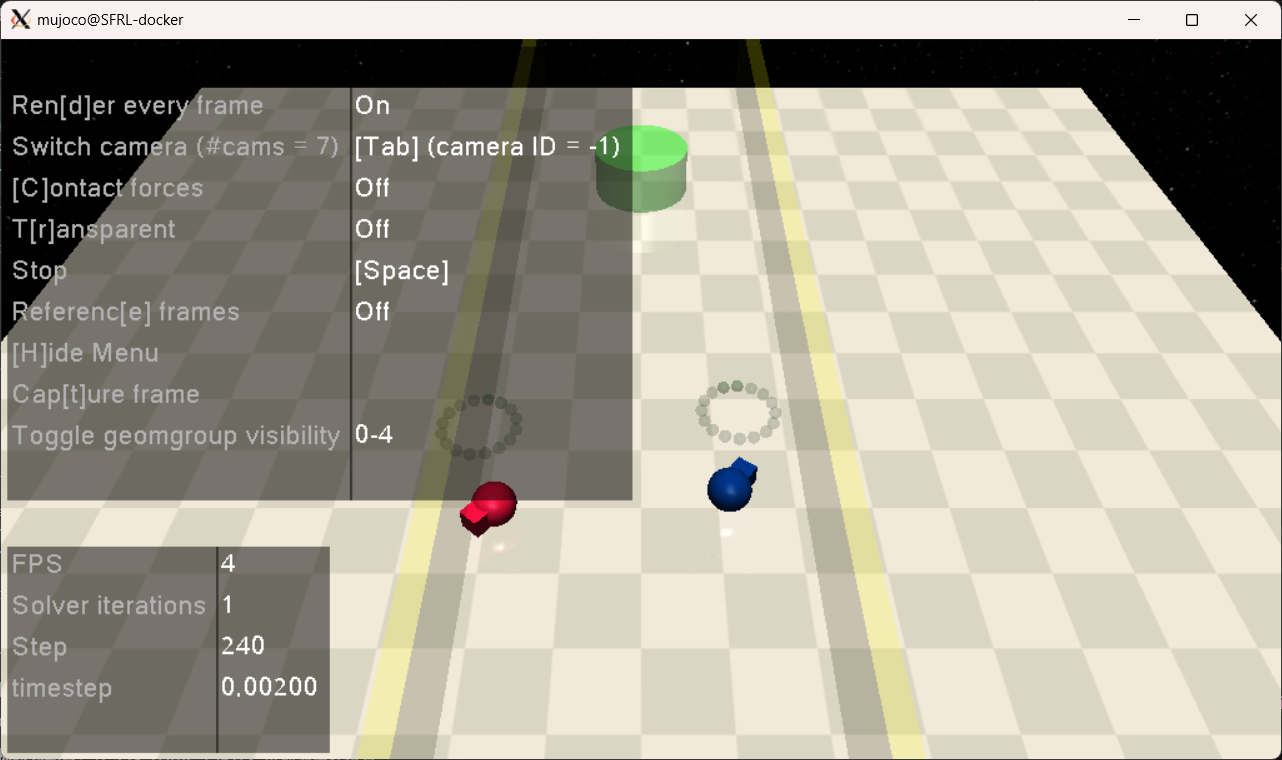
\includegraphics[width=1\linewidth]{images/rmp_env.png}
    \caption{Enter Caption}
    \label{fig:rmp_env}
\end{figure}

\subsection{评价指标}
为了全面评估算法性能，本文采用以下指标：
1）累计奖励（Total Reward）
统计策略在一个完整 episode 中获得的累计奖励：$R = \sum_t r_t$，反映策略整体行为质量。
2）安全代价（Collision Cost）
统计策略在一个完整 episode 中产生的累计安全代价：$C = \sum_t c_t$，用于评估系统安全性。
3）任务成功率（Success Rate）
成功率定义为：
\[SR = \frac{N_{success}}{N_{total}}\]
其中：$N_{success}$ 为成功到达目标且未发生碰撞的 episode 数；$N_{total}$ 为总测试 episode 数，该指标反映策略在复杂环境中的任务完成能力。

\subsubsection{奖励设置}
强化学习部分主要负责提供目标驱动和整体行为优化能力，因此设计了一系列奖励函数以引导策略学习合理的导航行为。
总奖励由多个子奖励组成：
\[r_t = r_{goal} + r_{progress} + r_{form} + r_{collision}\]
其中各部分定义如下。

\paragraph{目标导航奖励}
为了鼓励机器人不断接近目标位置，引入距离递减奖励：
\[r_{progress} = \beta (D_{last} - D_{now})\]
其中$D_{last}$为上一时刻机器人编队质心到目标的距离；$D_{now}$为当前时刻机器人编队质心到目标的距离；$\beta$为奖励权重系数。
当机器人朝目标移动时奖励为正；反之则为负，从而引导策略持续接近目标。
当机器人编队成功到达目标区域时，给予一次性的奖励：$r_{goal} = R_{goal}$，该奖励用于强化成功完成任务的行为。

\paragraph{编队保持奖励}
为保证多机器人系统在运动过程中维持期望的空间结构，本文设计如下编队保持奖励函数。设系统中共有 N 个机器人，其在二维平面中的位置为
\[
p = (p_0, p_1, \ldots, p_{N-1}), \quad p_i \in \mathbb{R}^2.
\]

当前编队形状由无向图 $\mathcal{G}=(\mathcal{V},\mathcal{E})$ 描述，其中每条边 $(i,j)\in\mathcal{E}$ 表示机器人 i 与机器人 j 之间需要保持期望距离 $d_{ij}^*$。该图结构与 GCPL 中用于构建编队保持节点的拓扑保持一致。

\subparagraph{距离保持奖励项}
对于任意约束边 $(i,j)$，定义其距离误差为
\[
e_{ij} = \left| |p_i - p_j|_2 - d_{ij}^* \right|.
\]

为了消除编队规模变化对奖励幅值的影响，采用所有边误差的平均值作为整体距离偏差：
\[
\bar{e} =
\begin{cases}
\frac{1}{|\mathcal{E}|} \displaystyle\sum_{(i,j)\in\mathcal{E}} e_{ij}, & |\mathcal{E}| > 0, \\
0, & |\mathcal{E}| = 0.
\end{cases}
\]

基于该平均误差，编队距离奖励定义为
\[
r_{\mathrm{dist}} = s_f \exp\left(-\frac{\bar{e}}{\tau}\right),
\]
其中 $s_f>0$ 为编队奖励尺度系数，$\tau>0$ 为距离容差参数，用于控制奖励对误差变化的敏感程度。当机器人间距离接近期望值时，$\bar{e}$ 较小，对应的奖励接近 $s_f$；而当编队结构被破坏时，奖励将随误差增大而快速衰减。

\subparagraph{形状辅助奖励项}

在部分编队形状中，仅依赖距离约束可能无法唯一确定整体朝向或宽度结构。为此，针对特定形状设计了额外的辅助奖励项 $r_{\mathrm{aux}}$。

在全连接网格（mesh）编队中，为避免结构发生整体旋转或镜像，引入边方向与期望方向的一致性奖励。对于边 ((i,j))，定义其单位方向向量为
\[
\hat{r}_{ij} = \frac{p_j - p_i}{|p_j - p_i|_2}.
\]

设 $\hat{r}^*$ 为期望的全局编队方向，则辅助奖励定义为
\[
r_{\mathrm{aux}} =
s_m \cdot
\frac{1}{|\mathcal{E}|}
\sum_{(i,j)\in\mathcal{E}}
\hat{r}_{ij}^\top \hat{r}^*,
\]
其中 $s_m>0$ 为方向一致性奖励权重。当编队边方向与期望方向对齐时，该项取得较高值，从而抑制编队在训练过程中发生无意义的旋转。

对于队列（line）编队，主要目标是保持机器人在某一主轴方向上排列，同时限制垂直方向的扩散。设编队主轴为 x 轴时，定义辅助奖励为
\[
r_{\mathrm{aux}} = - s_\ell , \mathrm{Var}( {p_{k,y}}),
\]
其中 $\mathrm{Var}(\cdot)$ 表示样本方差，$s*\ell>0$ 为宽度惩罚权重。该项通过惩罚机器人在垂直方向上的位置方差，使系统收敛到窄带状队列结构。若主轴为 y 轴，则对 x 坐标方差进行惩罚。

对于楔形（wedge）与圆形（circle）编队，其几何结构已由距离约束图 $\mathcal{E}$ 与目标距离 $d_{ij}^*$ 唯一确定，因此不额外引入辅助奖励项：
\[
r_{\mathrm{aux}} = 0.
\]

因此在每个时间步，对所有机器人采用共享的编队奖励信号：
\[
r_{\mathrm{form}}^k = r_{\mathrm{dist}} + r_{\mathrm{aux}},
\quad k = 0, \ldots, N-1.
\]

这种全局共享奖励设计与 MAPPO 的集中式训练机制相匹配，使各个智能体在优化自身策略时能够考虑整体编队结构的变化，从而学习到协同一致的群体行为。

\paragraph{碰撞惩罚}

如果机器人发生碰撞，则给予较大的负奖励：$r_{collision} = R_{collision}$。
该奖励用于强烈惩罚危险行为，促使策略避免碰撞。

\subsubsection{代价设置}

除奖励函数外，本文设计代价函数（Cost），用于度量系统在运行过程中产生的风险程度。该 cost 主要用于安全评估以及策略约束分析。
总安全代价定义为：
\[c_t = c_{hazard} + c_{robot}\]

障碍物接近代价：当机器人靠近环境障碍物时，产生风险代价：
\[c_{hazard} = \gamma (R_{hazard} - D_{hazard})\]
当$D_{hazard} < R_{hazard}$时产生代价，其中：$D_{hazard}$ 为机器人到最近障碍物的距离；$R_{hazard}$为危险距离阈值； $\gamma$ 为权重系数。
该代价函数呈 Barrier 型结构，当机器人靠近障碍物时迅速增加，从而刻画安全风险。

机器人间碰撞代价：
为了避免机器人之间的碰撞，引入机器人间安全距离代价：
\[c_i^{col} = \sum_{j\in\mathcal N_i} \beta_c \phi \big( d_{safe} - \|x_i - x_j\| \big)\]
其中： $d_{safe}$ 为机器人间安全距离；$\beta_c$ 为代价权重； $\phi(\cdot)$ 为ReLU 或 barrier 函数。
当机器人距离小于安全距离时，代价增加，从而反映系统风险。

\subsection{参数设置}
\begin{table}[htbp]
\centering
\small
\setlength{\tabcolsep}{6pt}
\renewcommand{\arraystretch}{1.2}
\begin{tabular}{p{0.22\linewidth} p{0.2\linewidth}|p{0.22\linewidth} p{0.2\linewidth}}
\hline
\multicolumn{2}{c|}{\textbf{训练参数}} & \multicolumn{2}{c}{\textbf{GCPL参数}} \\
\hline
\textbf{参数} & \textbf{参数大小} & \textbf{参数} & \textbf{参数大小} \\
\hline
总环境步数 & $10^8$ & 编队目标间距 & 0.5 \\
隐层宽度 & 512 &  直线编队轴向 & x \\
MLP层数 & 2 & 楔形半角（度） & 35.0 \\
折扣因子 & 0.96 & 期望编队方向 & [0.0, 1.0] \\
GAE系数$\lambda$ & 0.95 & 方向叶$\alpha_\theta$ & 1.0 \\
PPO裁剪系数 & 0.2 & 方向叶$\eta_\theta$ & 2.0 \\
mini-batch数量 & 1  & 方向叶度量$c_\theta$ & 10.0 \\
策略学习率 & $9\times10^{-5}$ & 碰撞安全半径 & 0.3 \\
价值学习率 & $5\times10^{-3}$ & 融合权重 & 1 \\

\hline
\end{tabular}
\caption{训练参数与GCPL参数}
\label{tab:train-rmp-cn}
\end{table}

\subsection{实验结果}
实验结果如图 ~\ref{fig:rmp_result}所示，可以看到在训练过程中，相比于 MAPPO，添加 GCPL 的方法 cost 明显降低，意味着机器人碰撞次数明显下降，安全性更好；同时reward 明显提升，在任务中表现更加出色。
同时，我们对训练结果进行了评估，分别用 MAPPO、MAPPO\_Lag 和我们的方法完成 20 轮次的任务，结果同样显示出我们的方法 reward 更高和 cost 更低，同时在20次任务中成功率更高。
\begin{figure*}[t]
\centering
\subfloat[reward]{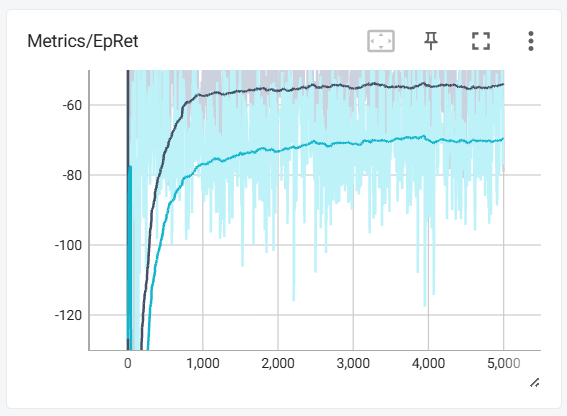
\includegraphics[height=4cm]{images/rmp_reward.png}}
\hfill
\subfloat[cost]{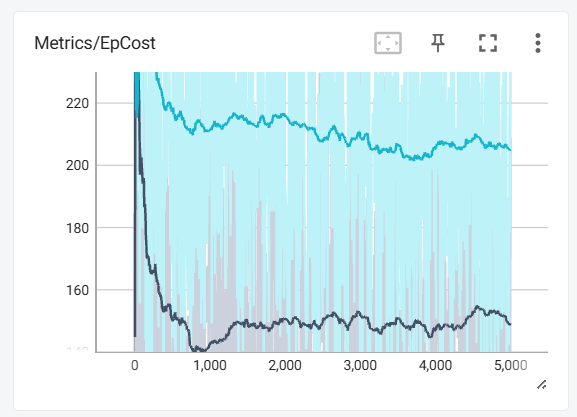
\includegraphics[height=4cm]{images/rmp_cost.png}}
\caption{GCPL 实验验证。其中蓝色表示mappo算法下的实验结果，黑色表示添加 GCPL 后的实验结果。(a) 训练过程中的reward (b) 训练过程产生的cost（表示碰撞次数）。}
\label{fig:rmp_result}
\end{figure*}

\begin{table}[htbp]
    \centering
    \caption{Experimental Results on SafetyPointMultiFormationGoal0-v0}
    \begin{tabular}{l c c c}
    \hline
    \textbf{Algorithm} & \textbf{Reward} & \textbf{Cost} & \textbf{Success Rate} \\
    \hline
    
    MAPPO      & $-21.46 \pm 3.43$ & $124.17 \pm 32.17$ & $0.13 \pm 0.09$ \\
    
    RMPflow  & $3.71 \pm 6.24$   & $22.85 \pm 19.37$  & $0.35 \pm 0.11$ \\
    
    MAPPO-Lag  & $-13.26 \pm 6.17$ & $125.96 \pm 34.05$ & $0.27 \pm 0.06$ \\

    GCPL  & $7.83 \pm 8.76$   & $27.15 \pm 14.51$  & $0.65 \pm 0.16$ \\
    
    \hline
    \end{tabular}
    \end{table}